\documentclass[12pt,a4paper,twoside,openright]{report}
\usepackage{tgtermes}
\usepackage[T1]{fontenc}
\usepackage{polski}
\usepackage[utf8]{inputenc}
\input glyphtounicode
\pdfgentounicode=1
\usepackage{amssymb}
\usepackage{amsmath}

\usepackage{placeins}
\usepackage{pdfpages}
\usepackage{csquotes}
\usepackage{graphicx}
\let\lll\undefined
\usepackage{indentfirst}
\usepackage{float}
\usepackage{tabularx}
\usepackage{hyperref}
\graphicspath{ {./img/} }
\usepackage[left=3.5cm,right=2cm,top=2.5cm,bottom=2.5cm]{geometry}
\usepackage{caption}
\captionsetup{font=small}

\newcommand{\mycaption}[2]{%
  \caption[#1]{#1\\ \footnotesize{#2}}%
}

\usepackage{datetime}
\usepackage{dirtree}
\renewcommand\DTstyle{\rmfamily}
\usepackage{listings}

\usepackage[defernumbers=true,
        locallabelwidth,
        backend=biber]{biblatex}

\addbibresource{bibliography.bib}

\pretocmd{\chapter}{\addtocontents{toc}{\protect\addvspace{-5pt}}}{}{}

\newcommand*{\typeprefix}{%
  \ifentrytype{article}{%%
  }{%
    \ifentrytype{book}{%%
    }{%
      www. % "other"
    }%
  }%
}

\DeclareFieldFormat{labelnumber}{\typeprefix #1}
\renewcommand*{\finentrypunct}{}

\lstset{
	basicstyle=\footnotesize\ttfamily,
    keepspaces=true,
    showstringspaces=false,
    commentstyle=\ttfamily,
    frame=single,
    aboveskip=18pt,
    belowskip=18pt,
    breaklines=true,
}
\raggedbottom
\newdate{date}{10}{06}{2019}
\usepackage[justification=centering]{caption}
\makeatletter
\def\@makechapterhead#1{%
\pagebreak
  \vspace*{120\p@}% <----------------- Space from top of page to Chapter #
  {\parindent \z@ \raggedright
    \ifnum \c@secnumdepth >\m@ne
        \huge\bfseries \@chapapp\space \thechapter. \Huge \bfseries #1\par\nobreak% <-- Chapter #
        \par\nobreak
        \vskip 24\p@% <-------------- Space between Chapter # and title
  }}
  
  \usepackage{titlesec}

    
\titlespacing{\section}{0pt}{18pt}{18pt}
\titlespacing{\subsection}{0pt}{18pt}{18pt}

\author{Karol Zygadło}
\linespread{1.3}




\begin{document}
    \begin{titlepage}
    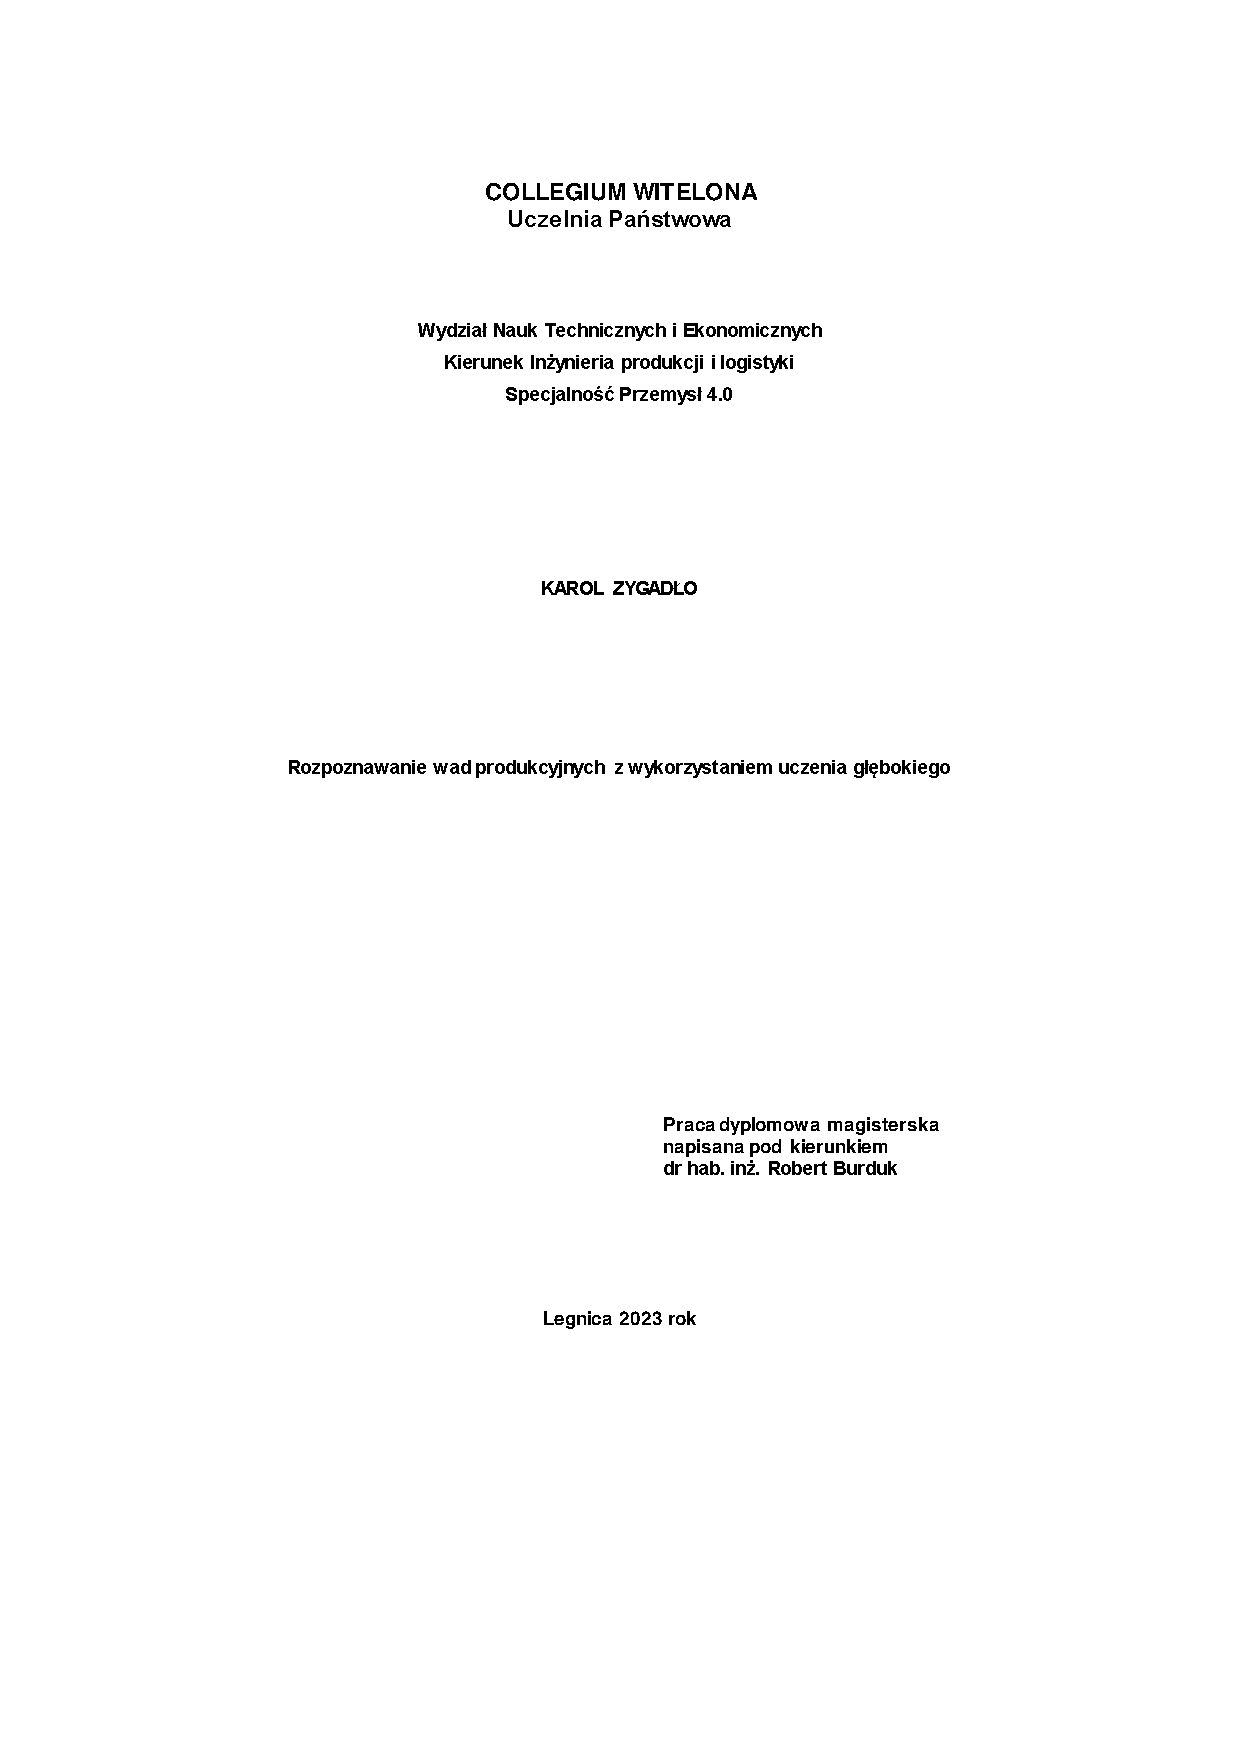
\includepdf{TitlePage.pdf}
    \end{titlepage}
\begingroup
    \let\clearpage\relax
    \tableofcontents
    
    \include{chapter1-wstęp}
    \chapter{Wprowadzenie}
\section{}
\endgroup

\medskip
\printbibliography[type=online, title={Netografia\footnote{Podane adresy zostały odwiedzone w maju 2020 roku. Nie ma gwarancji, że po tej dacie będą dalej aktywne lub poprawne.}}]
\printbibliography[type=book, title={Bibliografia}]
\lstlistoflistings
\listoffigures
\listoftables

\newpage

\chapter*{}
\centering\textbf{OŚWIADCZENIE\\[6mm]}
\raggedright
Oświadczam, że: 
\begin{enumerate}
    \item pracę niniejszą przygotowałem(am) samodzielnie; wszystkie dane, istotne myśli i sformułowania pochodzące 
z literatury (przytoczone dosłownie lub niedosłownie) są opatrzone odpowiednimi odsyłaczami; praca ta nie była 
w całości ani w części przez nikogo przedkładana do żadnej oceny i nie była publikowana;
    \item wyrażam zgodę / nie wyrażam zgody na udostępnianie mojej pracy dyplomowej. 
\end{enumerate}\\[10mm]
Data ..............................\\[15mm]


\centering
\hspace{200pt} ..............................................\\[0mm]
\hspace{200pt} imię i nazwisko\\[10mm]
\hspace{200pt} Stwierdzam autentyczność podpisu\\[5mm]
\hspace{200pt} .....................................................................\\[0mm]
\hspace{200pt} (podpis  pracownika i pieczątka Wydziału)\\[20mm]
 
 \raggedright
 * niepotrzebne skreślić
\end{document}